\section{Tools and Data}
Every year technology for generating and measuring particle collisions is improving. 
As a consequence, the amount of data increases drastically. The \ac{ATLAS} experiment
is one of the largest particle detector experiments currently operating at the 
CERN laboratory near Geneva. \ac{ATLAS} alone generates approximately 1 petabyte of raw
data every second from proton-proton collisions at the \ac{LHC}. In this analysis I will 
be studying proton-proton collisions produced by \ac{ATLAS} between 2015-2018, with a luminosity of 
$139.0fb^{-1}$ and center of mass energy of 13TeV. With amounts of data this large, data handling and 
storing is a big challenge. Therefore, taking advantage of sophisticated numerical tools 
and data frameworks is pivotal if scientific development is to keep up with technological development.
\\
In this section I will cover some tools and frameworks I have used to 
complete my analysis. Large amounts of details and explanations will not be covered. 
Instead, this section will highlight which tools were used and some motivation
for choosing them. Additionally, I will cover some details regarding the data
being used, both \ac{MC}-sumulations and real collision data.
\subsection{Monte Carlo Simulated Data}
Up to this point in the thesis, I have discussed two data sets: the measured collision data and the simulated data. 
As far as my relation to the latter data set, I have only used it directly in my analysis and have not been involved in 
production. The simulations applied in the creation of our simulated data set are all based on \acf{MC} simulations\footnote{For 
more information on \ac{MC} simulation, the reader is referred to \cite{raychaudhuri_introduction_2008}.}, produced 
by the popular frameworks like, \emph{$MadGraph5\_aMC@NLO$} and \emph{$Pythia\ 8.2$} \cite{alwall_automated_2014, sjostrand_introduction_2015}. 
Through simulation, we are able to (among other things); test our understanding of the detector, model the expected \ac{SM} background 
events in different regions or model new \ac{BSM} physics. The pipeline for producing simulated events, closely mimic the pipeline 
from real collision to data set. The pipeline for simulating collision events can be summarized in the following steps
\begin{itemize}
  \item \emph{Generate events}: Simulate each event in the collision, marking each event with the corresponding process (see section \ref{sec:bkg})
  \item \emph{Simulate detection of events}: Simulate the detection of each event in the different layers of the detector described in section \ref{subsec:Detector}
  \item \emph{Digitization}: Translate the interaction between the events and the detector to real signals
  \item \emph{Reconstruct events}: Go through the same steps applied to real collisions to reconstruct particles from signals
\end{itemize}
\subsection{The Simulated Signal}\label{subsec:signal}
As I have mentioned in previous sections I will be searching for a large range of signals, all related to the same
physics, but with different set of parameters. In figure \ref{fig:nrSignal} I have drawn a grid showing the different mass combinations 
searched for in this analysis. The figure shows the data set containing masses ranging from $m({\tilde{\chi}_1})\in[0,400]$
and $m({\tilde{\chi}_2})\in[100,800]$.\footnote{The chargino, $\tilde{\chi}^{\pm}_1$ and $\tilde{\chi}_2$ are mass degenerate, 
meaning they share the same mass.} In the beginning of my analysis I only received a subset (which will be referred to as the 
\emph{original} data set.) of the full signal set. In the figure I have marked the original data set with a white label in the top 
right corner of the box. The original signal set contains a total of 30 different mass combinations in the range from 
$m({\tilde{\chi}_1})\in[0,400]$ and $m({\tilde{\chi}_2})\in[400,800]$. In the full signal data set there are a total of 90 different 
mass combinations.
\\
Given that I received the original signal data set many months before receiving the full set, most of my results were found using the 
original set. Therefore, I choose to use the original data set to compare the models in performance, then finally use the full set 
when studying the models and finally comparing limits.
\begin{figure}
  \centering
  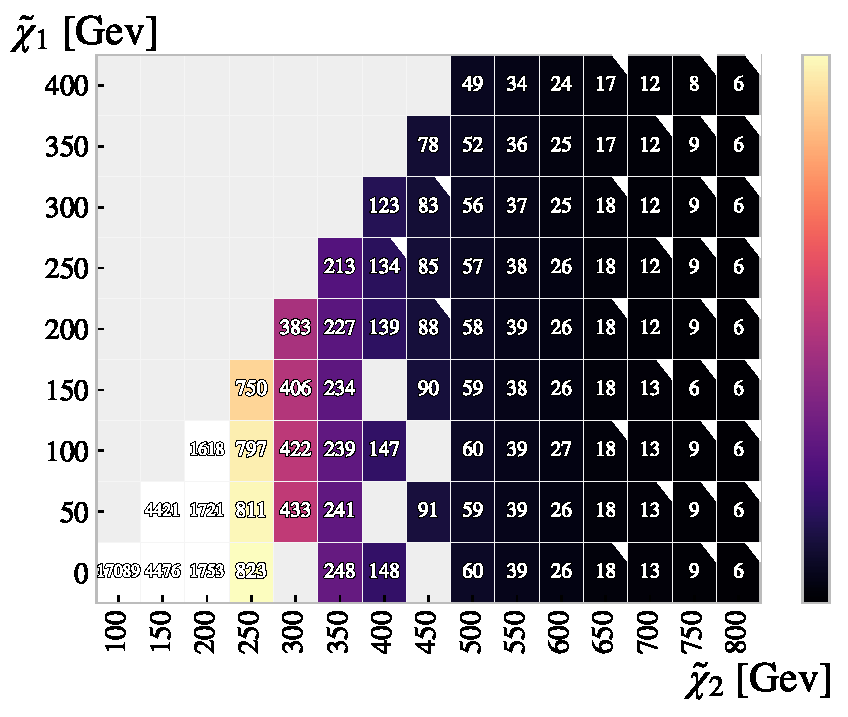
\includegraphics[width=0.85\textwidth]{Figures/MLResults/NN/SUSY/Grid/NrSignalEvents.pdf}
  \caption{A depiction of all mass combinations and their respective event count in the full signal data set.
  Additionally, a white corner has been added to all combinations which define the original signal set.}
  \label{fig:nrSignal}
\end{figure}
\subsection{ROOT}
In many aspects of my analysis, ranging from statistical analysis to plotting, I utilize the ROOT framework.
ROOT \cite{ROOT} is at its core a large $C{++}$ library and data structure made specifically for big data
analysis and computing, as well as data visualization. Today, all \ac{ATLAS} data is stored as a ROOT-file along
with more than 1 exabyte ($10^{12}$) of data worldwide. ROOT has many \ac{HPC} qualities which makes it ideal for particle
physics analysis which demands heavy computations. Additionally, many particle physics-specific packages
have been developed to make it an even better tool. Any function not already in library,
can easily be added in a \ac{HPC}-effective manner through $C{++}$.
\\
All distribution plots made for this thesis were created using ROOT. ROOT has implemented a highly intuitive and
effective \ac{API} for data comparison and visualization. ROOT allows for quick and direct 
comparison between data through an advanced graphical user interface. Additionally, a lot of
functionality for creating complex stacked histogram are implemented in the ROOT \ac{API}, such
as uncertainty calculations, ordering of histograms and statistical analysis tools. 
\subsection{Data Structure and Frameworks}
Both data sets analyzed in this thesis, the measured and simulated are originally (pre-processing) stored in ROOT, in the format of Ntuples. 
NTuples are ROOT objects, designed to store large amounts of data in a tabular form. They allow for non-symmetrical entries, meaning 
rows with different number of columns. The simulated and measured collision data are both stored in Ntuples, with a matrix like structure where the columns represent 
the variables/features, and the columns represent each event. Hence, allowing non-symmetrical entries is essential for the purpose of storing data on particle collisions, 
given that not all variables are relevant for all events. For example the $P_t$ of the 3 lepton in an event with 2 lepton final state, does not make sense.
\\
When starting preprocessing, I load the NTuples into another ROOT data structure called RDataFrame\footnote{For full 
documentation on RDataFrame, see $\href{https://root.cern/doc/master/classROOT\_1\_1RDataFrame.html}{https://root.cern/doc/master/classROOT\_1\_1RDataFrame.html}$ (Accessed 16.04.2023).}. 
RDataFrame allows for easy addition of new columns as well as filtering of events through native functionality. As 
a consequence I used RDataFrame to calculate all higher-level features such as the sum of $P_t$ ($H_t$), 
invariant mass of 3 leptons ($M_{lll}$) etc. An example is shown in the following section. 
\\
After all data handling was complete, I used ROOT's $AsNumpy$ function to translate the data frame as 
a Numpy object, which then allowed me to transform it to a Pandas-data frame \cite{Pandas}. This is done
because Pandas, like most \ac{ML}-tools work in a strict Python environment. Pandas, similarly to RDataFrame
includes many deep computational libraries, and is optimal for analysis of big data. When the full \ac{ML} 
pipeline (data-handling, training, validating etc.) is completed, the data is transformed back to RDataFrame, 
to take advantage of the plotting functionality in ROOT. The workflow of the method is visualized in figure 
\ref{fig:WF}.
\begin{figure}
  \centering
  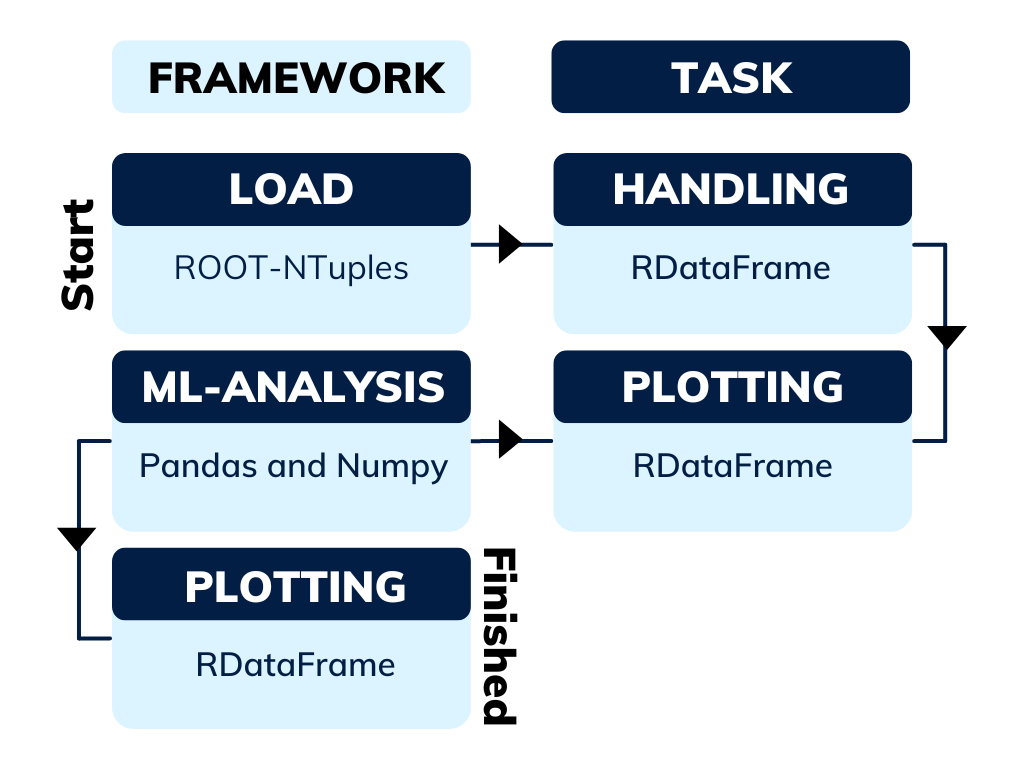
\includegraphics[width=0.7\textwidth]{Figures/Illustrations/TaskFlow.png}
  \vspace{-1cm}
  \caption{A visual summary of the workflow and frameworks used in the 
  computational analysis. }
  \label{fig:WF}
\end{figure}
\subsection{Computing Features in ROOT: Example}
In this section I will cover a simple example to highlight the steps taken in preparing the dataset 
I used in the analysis. As mentioned earlier, the two main frameworks used were RDataFrame and Pandas. 
In this example I will cover the case of a feature not already in the ROOT file, namely the trilepton
invariant mass. All loading of data is done using the ROOT framework and is quickly transformed into a 
RDataFrame. To effectively generate new features, we want to stay in ROOT and RDataFrame. Therefore,
we create our $C{++}$-file, \emph{helperfunction}. The helperfunction contains all additional 
ROOT functions that are used in the analysis and are not already native to ROOT. In the case 
of computing the trilepton invariant mass, the $C{++}$-function is created like shown in listing 
\ref{lst:mlll}.
\\
In listing \ref{lst:mlll}, we see a couple of measures taken to uphold to the ROOT environment. The first is 
the typecasting to $VecF\_t$. $VecF\_t$ is created to wrap floats in the native ROOT vector object, $RVec$. 
The same is done in other cases such as float and integers, $VecI\_t$ and $VecB\_t$. The second measure
was using $TLorentzVector$\footnote{For full documentation on $TLorentzVector$, see $\href{https://root.cern.ch/doc/master/classTLorentzVector.html}{https://root.cern.ch/doc/master/classTLorentzVector.html}$ (Accessed 16.04.2023).} 
to calculate the invariant mass. $TLorentzVector$ is a class native to ROOT with many built-in functions. In 
this case we use the class to create three vectors through the variables, $P_t$, $\eta$, $\phi$ and M. Then, 
through the $TLorentzVector$ class we can simply add all three vector together, and extract the invariant mass of the 3 leptons. 
\lstset{style=Cpp}
\begin{lstlisting}[caption={$C{++}$-function which implementes the calculation of $M_{lll}$.},captionpos=b, label={lst:mlll}]
// Compute the trilepton invariant mass 
float ComputeInvariantMass(VecF_t& pt, VecF_t& eta, VecF_t& phi, VecF_t& m) {
  TLorentzVector p1;
  TLorentzVector p2;
  TLorentzVector p3;
  p1.SetPtEtaPhiM(pt[0], eta[0], phi[0], m[0]);
  p2.SetPtEtaPhiM(pt[1], eta[1], phi[1], m[1]);
  p3.SetPtEtaPhiM(pt[2], eta[2], phi[2], m[2]);
  return (p1 + p2 + p3).M();
}
\end{lstlisting}
With a helper function created in $C{++}$ we can move over to a Python and RDataFrame environment
for calculation and plotting. In the code written in listing \ref{lst:df_mlll}, I have shown a simple example 
of loading new $C{++}$-functions, filtering out bad events, calculating new features and adding said 
features to a histogram. The first three lines of code both process and include the helperfunctions 
into the ROOT framework. Then I loop over all keys in the data frame, which in my case
are the different channels (i.e diboson, $t\bar{t}$ etc.). For each channel I select 'good' events,
based on the criteria from section \ref{subsec:Cuts}. Then, I use RDataFrame's $Define$ function to calculate
and add a new feature using our $ComputeInvariantMass$-function. Finally, I save the feature as ROOT object called 
$Histo1D$, which I later plot using ROOT plotting \ac{API}'s. In this example I chose the trilepton invariant mass, 
but in the analysis all high-level features were calculated using a similar method. 
\lstset{style=Python}
\begin{lstlisting}[caption={Python-file for calling dataframe and calculating $M_{lll}$.},captionpos=b, label={lst:df_mlll}]
R.gROOT.ProcessLine(".L helperFunctions.cxx+");
R.gInterpreter.Declare('#include "helperFunctions.h"') 
R.gSystem.Load("helperFunctions_cxx.so")

for k in df.keys():
    # Define good leptons
    isGoodLepton = "feature1 < cut1 && feature2 >= cut2"

    # Define good leptons in dataframe
    df[k] = df[k].Define("isGoodLepton",isGoodLepton)

    # Define number of good leptons
    df[k] = df[k].Define("nGoodLeptons","ROOT::VecOps::Sum(isGoodLepton)")

    # Demand 3 good leptons 
    df[k] = df[k].Filter("nGoodLeptons == 3")

    # Define Invariant Mass (lll)
    df[k] = df[k].Define("mlll","ComputeInvariantMass(lepPt[isGoodLepton], 
                                                      lepEta[isGoodLepton], 
                                                      lepPhi[isGoodLepton], 
                                                      lepM[isGoodLepton])")
    # Add to histogram
    histo["mlll_%s"%k] = df[k].Histo1D(("mlll_%s"%k,
                                        "mlll_%s"%k,40,50,500),
                                        "mlll",
                                        "wgt_SG")     
\end{lstlisting}



